
\documentclass[11pt]{article}
 
\usepackage[margin=1in]{geometry} 
\usepackage{amsmath,amsthm,amssymb}
\usepackage{graphicx} 
\usepackage{blkarray}
\usepackage{amsmath}




\newcommand{\N}{\mathbb{N}}
\newcommand{\Z}{\mathbb{Z}}
 
\newenvironment{problem}[2][Problem]{\begin{trivlist}
\item[\hskip \labelsep {\bfseries #1}\hskip \labelsep {\bfseries #2.}]}{\end{trivlist}}
\newenvironment{lemma}[2][Lemma]{\begin{trivlist}
\item[\hskip \labelsep {\bfseries #1}\hskip \labelsep {\bfseries #2.}]}{\end{trivlist}}
\newenvironment{exercise}[2][Exercise]{\begin{trivlist}
\item[\hskip \labelsep {\bfseries #1}\hskip \labelsep {\bfseries #2.}]}{\end{trivlist}}

\newenvironment{question}[2][Question]{\begin{trivlist}
\item[\hskip \labelsep {\bfseries #1}\hskip \labelsep {\bfseries #2.}]}{\end{trivlist}}
\newenvironment{corollary}[2][Corollary]{\begin{trivlist}
\item[\hskip \labelsep {\bfseries #1}\hskip \labelsep {\bfseries #2.}]}{\end{trivlist}}

\usepackage{indentfirst}
\linespread{1.2}     % 调整间距
\setlength{\parindent}{0pt}

\begin{document}

 
% --------------------------------------------------------------
%                         Start here
% --------------------------------------------------------------
 
\title{Homework 7 DS-GA 1002 }%replace X with the appropriate number
\author{Yuhao Zhao\\ %replace with your name
Yz3085} %if necessary, replace with your course title
 
\maketitle
\begin{problem}{1}
\end{problem}
a) No. If we do not reject the Null hypothesis, it means we just don't have enough information to discard it. It does not mean we consider it right or likely.\\

b)No. If we take a frequentist perspective , the hypothesis is deterministic. So it's either true or not, there is no probability associated with the hypothesis. \\

c) For exploratory phase, we want don't want to reject hypothesis easily. We want to minimize the probability of reject the Null when it's true which is the type I error. Then we want a small reject region thus a small size and small power. \\

d) For determining the significance of some effect, we want to maximize the power, thus we need a large size and large power.\\

e) When we apply Bonferroni's method to a very large number of hypothesis,  for a fixed significance level $\alpha$,we reject the ith null hypothesis if $p_i \leq \frac{\alpha}{n}$ .This means it's very hard to reject the Null hypothesis for large n.  \\

\begin{problem}{2}
\end{problem}
a) We want to test whether the car will have problem for the first time or not in one year on average. The time until the car breaks down for the first time follows a exponential distribution $\sim exp(\lambda)$.\\ 
The mean of the distribution is $\frac{1}{\lambda}$ which is  the expected time when the car first break. Therefore we want to test whether $\frac{1}{\lambda} >1$\\
Therefore, the hypothesis could be:\\ $H_0: \lambda > 1, \\H_A: \lambda \leq 1$\\
The test statistic is $T = max_{1\leq i\leq n} t_i$, and we reject the null hypothesis when $T\geq \eta$\\

b) $\beta(\lambda,n,\eta)=P(T \geq \eta) =  1 - P(max(t_i)< \eta) =1 - P(t_i<\eta)^n =  1 - (1 - e^{-\lambda \eta})^n$\\

c) 

\begin{centering}
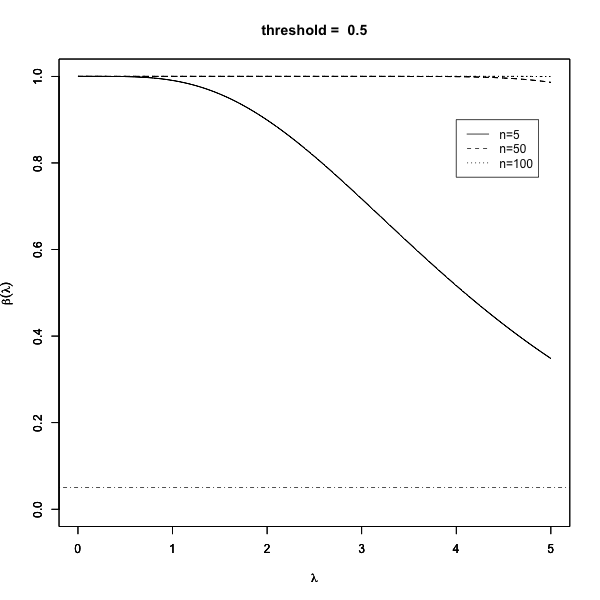
\includegraphics[height = 3.3in]{Q1} 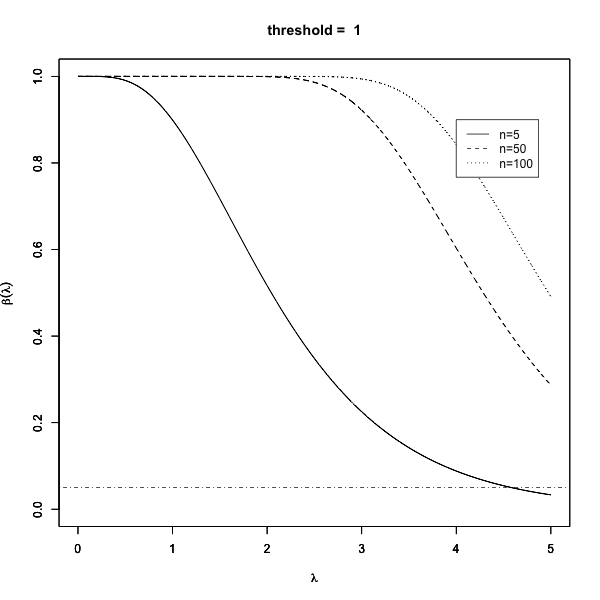
\includegraphics[height = 3.3in]{Q2} 
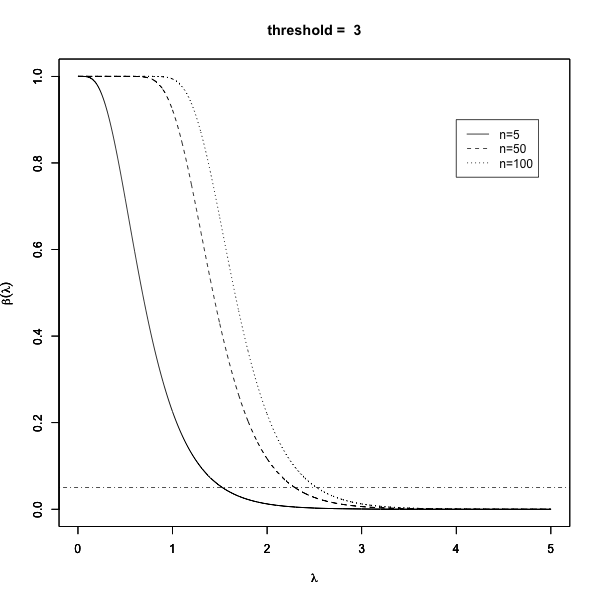
\includegraphics[height = 3.3in]{Q6} 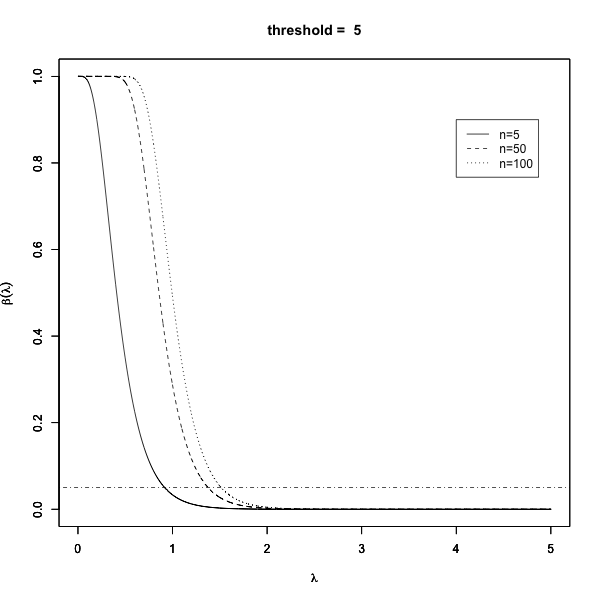
\includegraphics[height = 3.3in]{Q10} 
\end{centering}
From the plots, we want the power to be 1where $\lambda < 1$ and 0 where $\lambda >1$. For small values of threshold(0.5 and 1), the level is very high but the power is high. For large threshold(3 and 5) for small value of n, the test has a small level and large power. But for large n, the test has relatively large level and large power. 

\pagebreak
\begin{problem}{3}
\end{problem}
a). The null hypothesis could be:\\
 $H_0$: There is no length difference in ears for most of people.\\ 
 $H_A$: The left ear of most people is longer than the right ear.\\
 
b) The size of the test is the probability of making a type one error.\\ In this case is $P(T \geq \eta) = \frac{1}{2^{10}} \sum_{k = \eta}^{10} {10 \choose k}$\\

c) From the data, 6 sample have longer left ear than right ear. So $T = 6$.\\ The p-value $P(T \geq 7) =\frac{1}{2^{10}} \sum_{k = 7}^{10} {10 \choose k} \approx 0.171874 $

\begin{problem}{4}
\end{problem}
 a) The output using 10000 permutations are: 
 \begin{verbatim}
 Difference in sample mean is 19.217991311
 Difference in sample median is 21.5
 p value for difference in sample mean is 0.00113
 p value for difference in sample median is 0.00228
 p value for difference in sample mean is 0.00106
 p value for difference in sample median is 0.00236
 p value for difference in sample mean is 0.00114
 p value for difference in sample median is 0.00192
 \end{verbatim}
 The p-values for the difference of the sample median are 0.00228, 0.00236 and 0.00192\\
 
 b) 
 
  \begin{centering}
 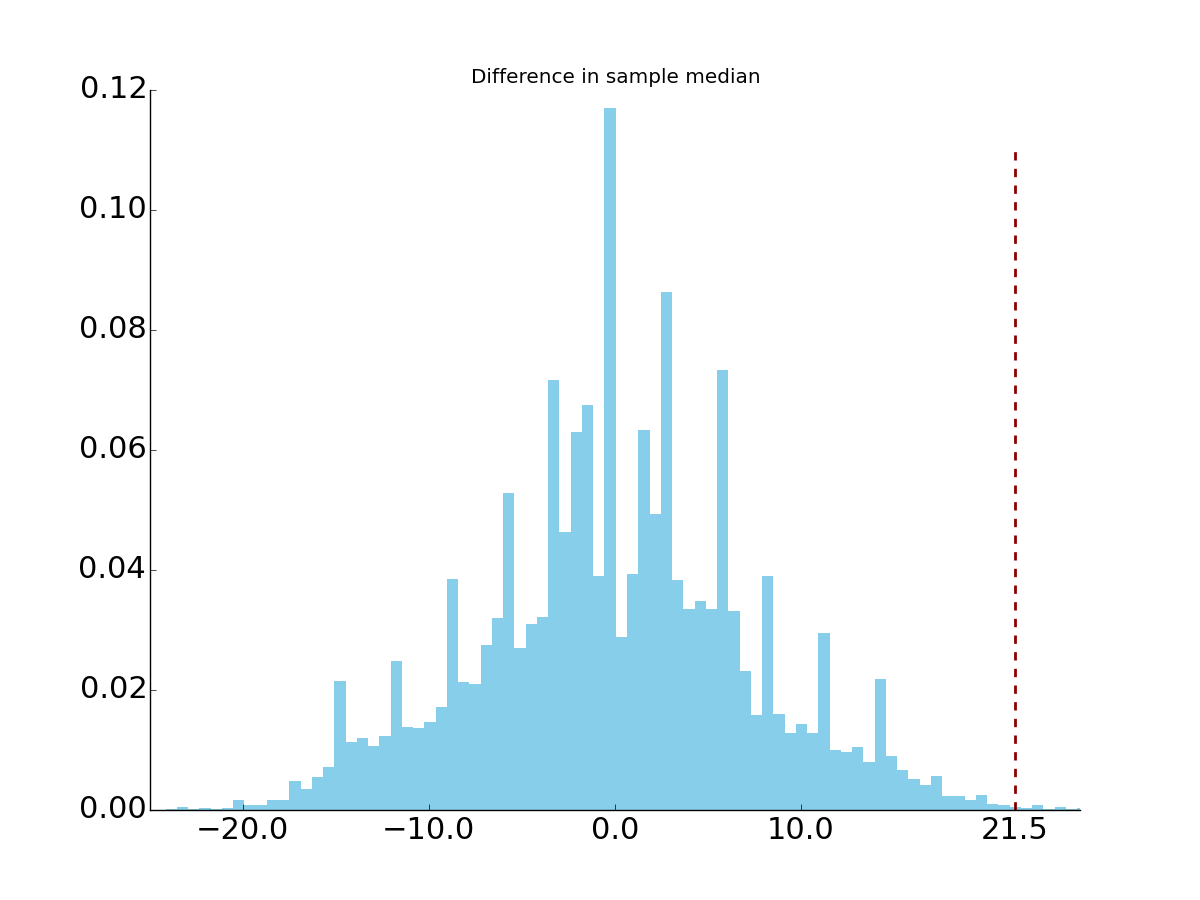
\includegraphics[height =2.5in]{figure_2}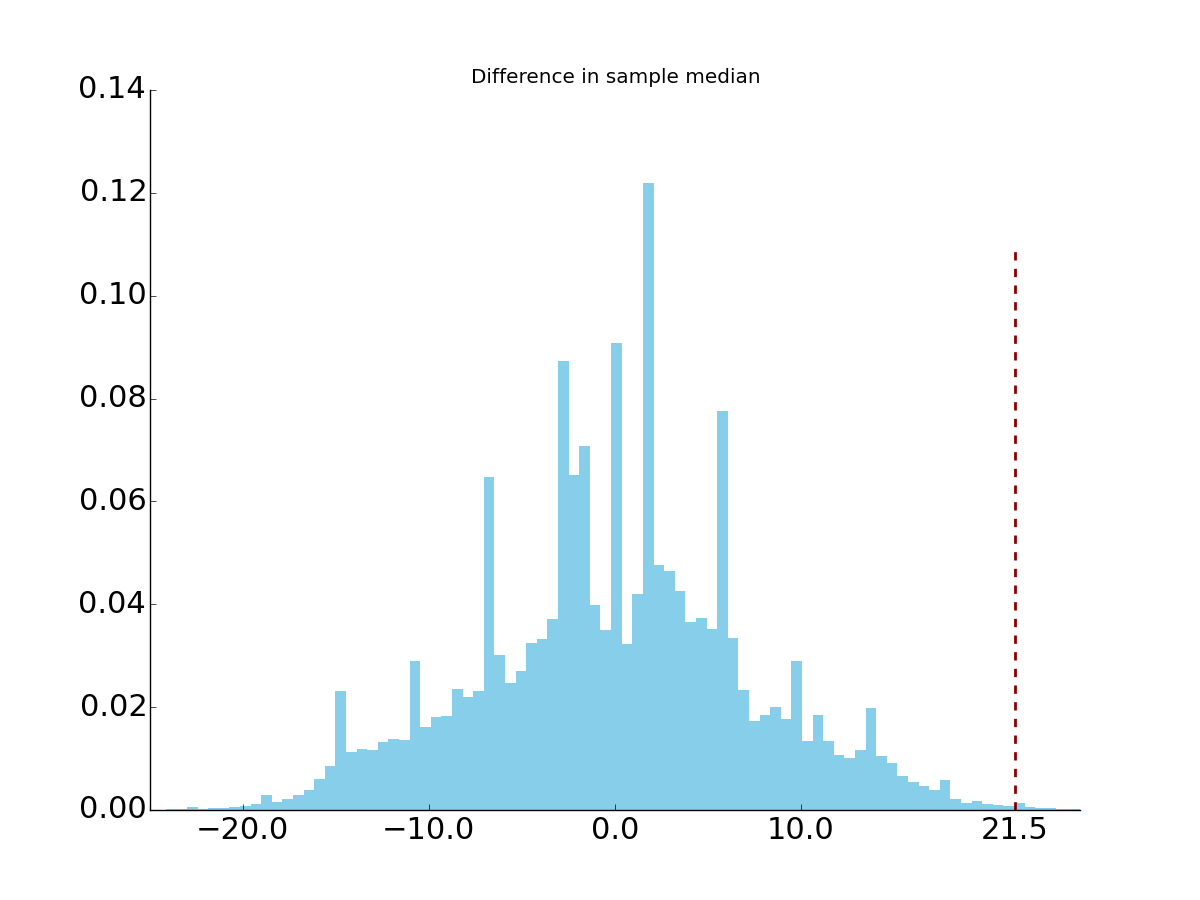
\includegraphics[height =2.5in]{figure_4}\\ 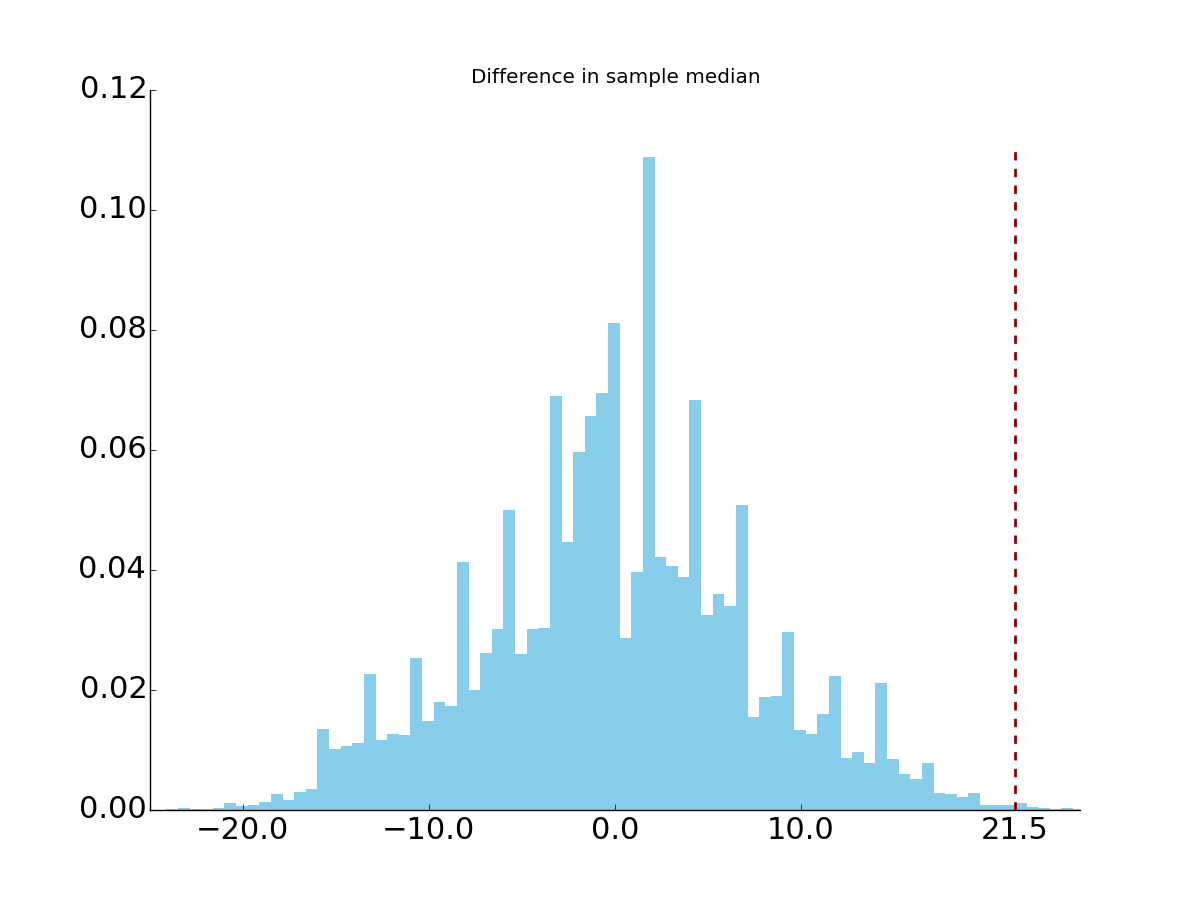
\includegraphics[height =2.5in]{figure_6}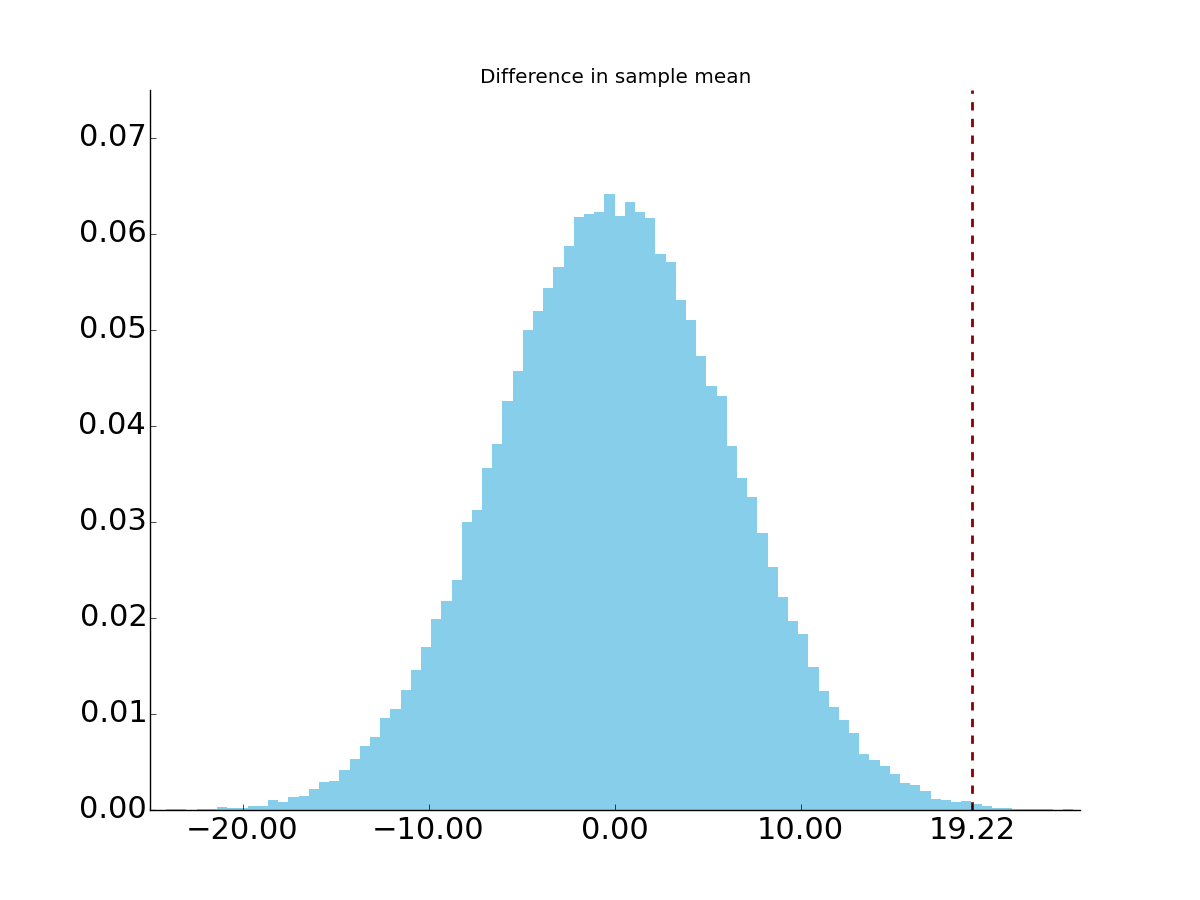
\includegraphics[height =2.5in]{figure_1}\\
 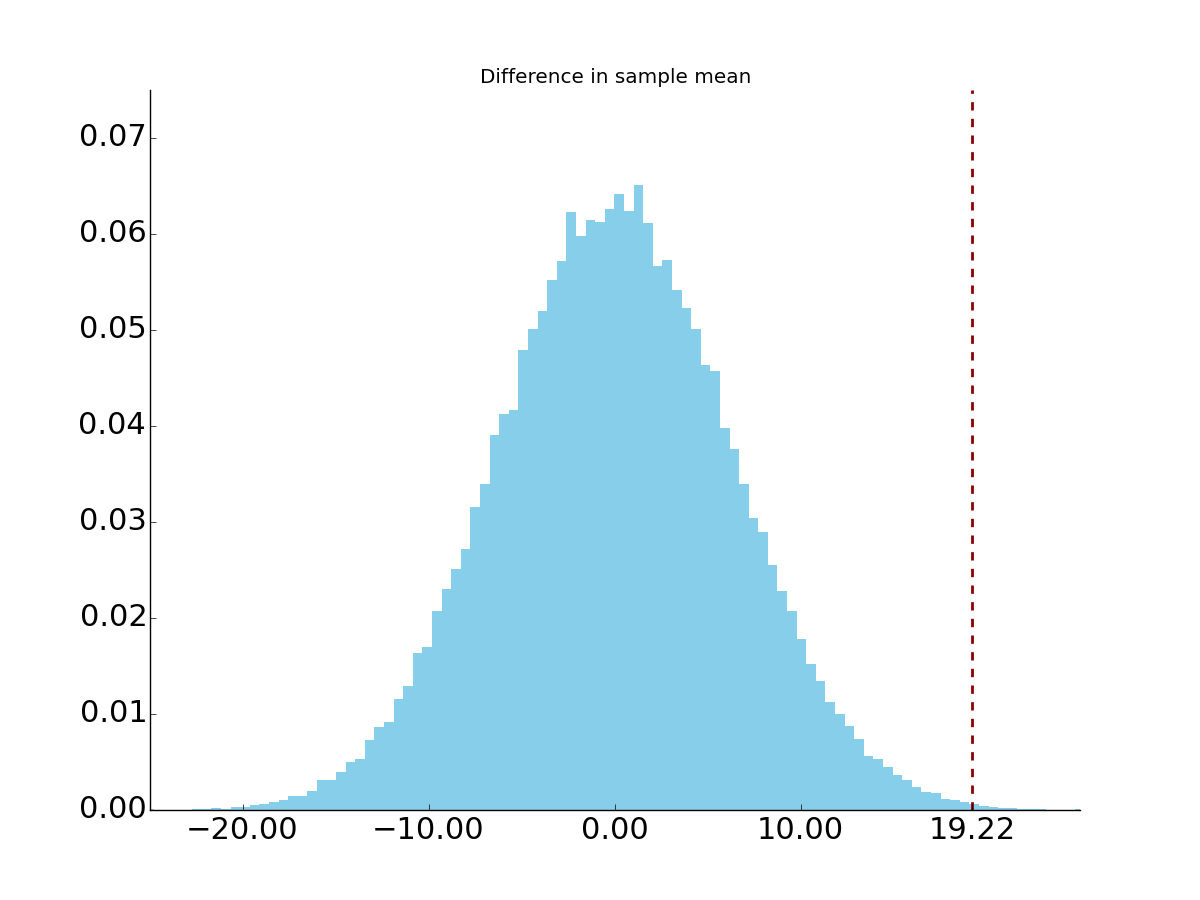
\includegraphics[height =2.5in]{figure_3}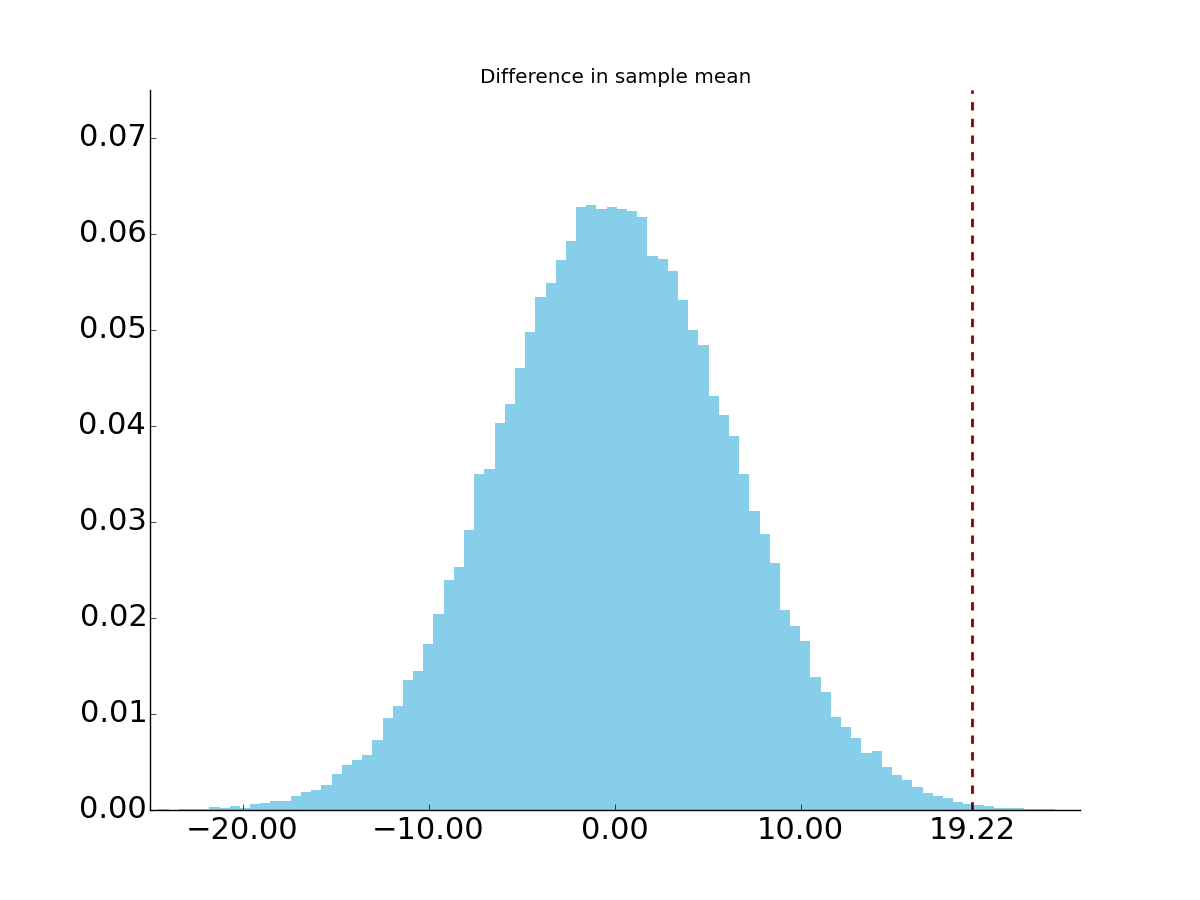
\includegraphics[height =2.5in]{figure_5}
 \end{centering}
 
 The p-values for the difference of median is a bit larger than that for mean. It's also clear from the histogram that the distribution of difference of median has heavier tails than that for the mean. Even though the median is a robust statistics, it does not guarantee a smaller p-value than the sample mean. In this data set, we don't have too much outliers, therefore it still make sense that  the mean has a smaller p-values.

\begin{problem}{5}
\end{problem}
 The essay \textit{Why most published research findings  are false} by John Ioannidis, illustrate the point that most current published research work are not correct because they should not be interpreted based only on p-values.The probability that a research finding is indeed true depends on the prior probability of the theory  being true, the statistical power of the test, and the statistical significance level. By analyzing the 2 $\times$ 2 Research Findings and True Relationships table, it can be shown that a research finding is more likely true than  false  if the power times  the ratio of the number of “true relationships” to “no relationships”  is larger than the significance level. What's more the bias and the repetition of testing by different teams studying the same problem may result even smaller probabilities of the research findings being indeed true. 





\end{document}